\documentclass[%
aip,
jmp,
reprint,
floatfix,
nofootinbib
]{revtex4-1}

\usepackage{graphicx}% Include figure files
\usepackage{dcolumn}% Align table columns on decimal point
\usepackage{bm}% bold math
\usepackage{float}
\usepackage{siunitx}
\usepackage{hyperref}
\usepackage{listings}
\usepackage[english]{babel}
\usepackage[]{natbib}
\bibliographystyle{astron}
\usepackage[utf8]{inputenc}
\usepackage{ gensymb }

\mathchardef\mhyphen="2D

\renewcommand{\arraystretch}{1.3} % Changes the height of tables
\DeclareSIUnit\year{yr}
\DeclareSIUnit\parsec{pc}
\DeclareSIUnit\day{d}



\begin{document}
	
	\title[Light-Curve of DQ Cephei]{The Light-Curve of DQ Cephei}
	
	\author{Lucas, Miles}
	\author{Brandon, John}
	\affiliation{Iowa State University}
	
	\date{\today}
	
	
% Write here a short abstract (1 paragraph) describing what you achieved in this lab.

	\begin{abstract}
	We sought to characterize the light-curve of $\delta$-scuti star DQ Cephei in its fundamental mode. We took approximately five hours of images every 25 seconds during two different observation sessions in 2017. We performed differential photometry using HD 235411 \SI{9.76\pm.03}{V} and HD 200017 \SI{8.20\pm.01}{V} as references. We used a Lomb-Scargle periodogram with a one-term Fourier model for time-series analysis and determined the period of DQ Cep to be \SI{0.0789\pm.0022}{\day}. Using the same model we estimate the amplitude to be \SIrange{7.26\pm.20}{7.30\pm.20}{V} ($\Delta$ = \SI{.0367\pm.0010}{mag}). However, due to the limits of our telescope and CCD, large variations in differential photometry results do not give much confidence to our amplitude estimates. 
		
	\end{abstract}
	
	\maketitle
%________________________________________________________________________
	
%	Write here a summary of the goals of this lab. Be brief – do not exceed the end of the first page.

	\section{Introduction}
	
	The goal of this report is to characterize the light-curve of $\delta$-scuti star DQ Cephei. $\delta$-scuti stars are a subclass of cepheids and exist on the instability strip. The cause for the variations of cepheids are due to the change in temperature and radius. These changes are self-excited by the second ionization of helium \citep{1963ApJ...138..487C} which, when compressed, increased the opacity of the star. As opacity increases, the radiation energy is blocked by the opacity. This causes a pressure which pushes the outer layers back out. This cycle continues regularly, causing the fundamental mode of oscillation \citep{1935PASP...47..232F}. 
	
	DQ Cephei falls into the class of low-amplitude-delta-scuti (LADS) which are classified with amplitude less than \SI{0.1}{mag}. These stars typically exhibit multivariability due to non-radial pulsation \citep{1937LicOB..18...77F, 1938ApJ....87..133S}. Another mode of pulsation are asymmetric surface instabilities. These overtones are usually quite hard to notice in comparison to the fundamental mode, with longer periods and even slighter amplitudes. High-amplitude-$\delta$-scuti (HADS) appear like small-period cepheids and are often termed as "dwarf-cepheids". In general, we expect these types of stars to behave similar to RR Lyrae variable stars. For more information on HADS seek \citet{1997PASP..109.1221M}. 
	
	The significance of finding the period from the light-curve of this star is to test the limits of our physical setup and to offer more data for the period-luminosity relationship of $delta$-scuti types.
	
	\begin{table*}[t]
		\centering
		\label{tab:info}
		
\caption{Information about target and reference stars}
\begin{tabular}{rrrrrr}
	\hline
	Object & Type &            RA &                DEC &                      V &                        Ref \\ \hline\hline
	DQ Cep &  *dS & 20 57 48.6082 & \ang{55;29;15.602} & \SIrange{7.40}{7.48}{} & \cite{1971GCVS3.C......0K} \\
	HD 235411 &    * & 20 57 31.1094 & \ang{55;31;38.697} &     \SI{9.76\pm0.03}{} &  \cite{2000AA...355L..27H} \\
	HD 200017 &    * & 20 58 27.2026 & \ang{55;39;00.459} &     \SI{8.20\pm0.01}{} &  \cite{2000AA...355L..27H} \\ \hline
\end{tabular}
	\end{table*}

	\begin{figure}
		\centering
		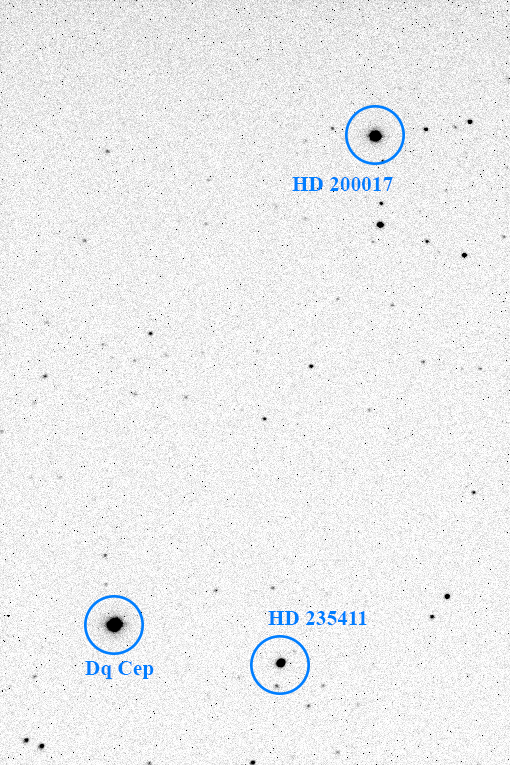
\includegraphics[width=.8\linewidth]{figs/map.png}
		\caption{Target image from our SBIG ST-402ME with the focal length extender. The image scale is about \SI{200}{\arcsecond} on the short side and about \SI{200}{\arcsecond} on the long side. We can see how the CCD has to be oriented correctly to include all stars.}
		\label{fig:map}
	\end{figure}
	
%________________________________________________________________________	

%	Describe your telescope and camera setup. For the first lab you should describe the setup in more details. Subsequent labs can refer to the procedure described in the first lab, and focus more on the data acquisition itself. Important details to write include: which stars have been observed, which filters were used (BVI), what exposure times and what calibration procedures have been followed (e.g., dark frames acquisition, photometric standards observed, etc.). Mention also the observing conditions (weather, moon presence, temperature, etc.). You should include the observing log appendix A (a table or a scan of a hardcopy). This section can be as long as necessary, but you should strive for brevity (you can refer to the lab guide to avoid repeating all steps, but make sure you explain anything you did differently, problems encountered, etc.). Use tables to summarize information clearly.

	\section{Data Acquisition and Setup}
	Observations were made on \date{27 September 2017} and \date{18 October 2017} at the Zaffarano Hall observation deck in Ames, Iowa (\ang{-93.64734}, \ang{42.02996}, \SI{342}{\meter}). Both nights had clear viewing and the ambient temperature was around \SI{13}{\degreeCelsius} for the first viewing and \SIrange{16}{4}{\degreeCelsius}. The moon had little to no effect on our sight either night due to the target position being \ang{107} away. Observations were made using a Meade 8" reflector telescope with a 2x focal length extender and an SBIG ST-402ME CCD camera with internal V, B, and I filters. 
	
	Setting up the telescope was the same as previous observations made with the 8" Meade telescope at Zaffarano Hall. \date{27 September 2017} was the trial night to determine whether DQ Cep would be visible and if the difference in magnitude could be seen. 
	
	A lot of time was spent locating the star of interest and orienting the camera. The method we found best for use with our specific Meade telescope was to slew to SAO 33047 and refernce a star chart to see where it sits in relation to DQ Cep and also SAO 33050. Now, slew to SAO 33050 and notice which direction the telescope slews. This will define polar axis in relation to the star chart. Then, we found similar triangle and were able to orient ourselves correctly on both axes compared to the star chart and then slewed to DQ Cep. Using the focal length extender was necessary to get both of our reference stars in the frame. This also depends on the orientation of the CCD, so we made sure to rotate the CCD on the mount so that all stars are in the image. This is shown in \autoref{fig:map}. 
	
	After focusing and determining our exposure time, we took 100 frames with \SI{15}{\second} exposures and a \SI{10}{\second} pause in between each frame. This pause is vital to allow realigning as the stars and mount fall out of alignment as the Earth rotates. In general we noticed about every 10 frames a small movement was necessary to keep all sources fully in frame.
	
	The observations on \date{18 October 2017} were meant to gather as much data as possible. With a previously stated period of \SI{.0789}{\day} (\SI{1.89}{\hour}) \citep{1971GCVS3.C......0K}, we sought to get data over two full periods, so four hours of observations. One of us started observations around 8:00 pm and started taking 500 frames. At 10:00 pm we switched observers and ran until the end of the night. In all we gathered 483 science frames and 5 dark frames.
	
	
	
%________________________________________________________________________

%Describe what you did to analyze the data. For the first lab this section will be minimal. For subsequent labs you should describe in detail the steps you did to analyze the data.  If applicable you can attach the code you used to analyze the data in Appendix B (either a log of your IDL section, or the code of any scripts you wrote). You can also attach screenshots of your computer session if it helps your discussion. Include tables of raw data in this section. The goal of this section is to describe unambiguously what you did to derive your final images and measured quantities from the raw data. Again be brief but complete (use as much space as you need).
	\section{Data Analysis}
	
	Our data analysis pipeline has two major parts. The first is the differential photometry of all 583 frames and the second is using a Lomb-Scargle periodogram to determine the optimal period for fit. 
	
	\subsection{Photometry}
	
	For differential photometry we used AstroImageJ (AIJ) due to its ability to process large stacks of images. We used multi-aperture mode and set the reference magnitudes according to \autoref{tab:info}. We tried using the automatic mode that would use image analysis to place the apertures on every frame, but since the position of the stars is changing in every frame, the automatic processing failed. That left us with one-click mode where, after placing initial apertures, we could move through each frame and click on the same reference point to place all apertures. 
	
	For our apertures, we used the same for each object, with circular inner aperture with radius 10 pixels and outer sky annulus with inner radius 15 pixels and outer radius 25 pixels. In AIJ we could set the multi-aperture photometry to reference the image header for the electron gain, which was nice. The algorithm AIJ uses is a sky-median subtraction, which takes the median value of the sky annulus times the area and subtracts it from the integrated aperture sum of the target.

	We ended up with two results tables for each observation date, which we concatenated together into one large CSV table which is stored at \href{https://github.com/mileslucas/astro344l/blob/master/project/data/full_data.csv}{this github page}.
	
	\subsection{Light-curve fitting}
	
	In order to create a light-curve from this data, we needed to phase-fold our data and create a model based off an optimal period. If our data was a signal with a sampling frequency, we could do a fast fourier-transform (FFT) and find the fundamental frequency. However, our data is not regularly sampled and we seek a different solution, which was proposed by \citet{1976Ap&SS..39..447L} and improved by \citet{1982ApJ...263..835S} is known as the Lomb-Scargle process. This process creates a power for each frequency using combinations of Fourier series, some of which can be approximated in a $O(N \log{M})$ implementation \citep{1989ApJ...338..277P} where there are $N$ data points and $M$ frequencies to sample. The original implementation runs in $O(N M)$ and is also limited to single term truncated Fourier series.	
	
	For determining the optimal period, we used Astropy's Lomb-Scargle methods for fitting and modeling our data. We modeled using a single term Fourier series (sine wave) and allowed the package to automatically parameterize the method. The power is normalized with a reference $\chi^2$ value 
	\begin{equation}
	P_X(f) = \frac{\chi^2_{ref} - \chi^2(f)}{\chi^2_{ref}}
	\end{equation}
	this value is limited to $0<=P_X<=1$. What this means is that the highest power frequency will create a model that minimizes in a weighted-least-squares fashion the residuals between the model and the data. So, as we find our best period, we can find the confidence interval using the standard error of the best fit model ($Y^*$) to the data ($Y$).
	\begin{equation}
	s = \cdot\sqrt{\frac{\sum_i{(Y^*_i-Y_i)^2}}{N-2}}
	\end{equation}
	Using least-squares error propagation shows that the uncertainty of the period is
	\begin{equation}
	\sigma_T = \frac{d}{d \omega}(\frac{1}{\omega})\cdot \omega s = \frac{s}{\omega}
	\end{equation}
	
	Even though our data is more regularly sampled than an RR-Lyrae would be, we chose the Lomb-Scargle over a classic periodogram. Because of this, we can treat both observation nights as one dataset with a 21 day gap and helps smooth out the irregular sampling rate caused by small interruptions on the second observation night.
	
	 We wrapped this method with Pandas DataFrames to read our CSV table and using matplotlib to present our data. All of the analysis was done in a jupyter notebook at \href{https://github.com/mileslucas/astro344l/blob/master/project/src/project.ipynb}{this github page}. For more information about Lomb-Scargle analysis, please reference \citet{2017arXiv170309824V}.


%________________________________________________________________________
	
%	Describe in detail the results you obtained from the quantitative analysis of your data, as explained in the lab guide.
	\section{Results}
	
	The differential photometry yielded the magnitudes, with errors, shown in \autoref{fig:raw}. The plot is broken to show both observation nights easily side by side. The time is referenced as the time since the first image was taken. 
	
	The Lomb-Scargle periodogram is shown in \autoref{fig:power}. We can see a clear peak around \SI{0.528\pm .015}{\per \hour}. This corresponds to a period of \SI{1.892\pm.053}{\hour} or \SI{0.0789\pm.0022}{\day}. We use this to fold all of our data and use Astropy's single-term model to show the fit in \autoref{fig:fit}. From this model, we can say the magnitude range for DQ Cep is \SIrange{7.26\pm.20}{7.30\pm.20}{mag} (\SI{.0367\pm.0010}{mag}), while the raw data has a range of \SIrange{7.24}{7.33}{mag} (\SI{.09}{mag}).
	 \begin{figure}[t]
	 	\centering
	 	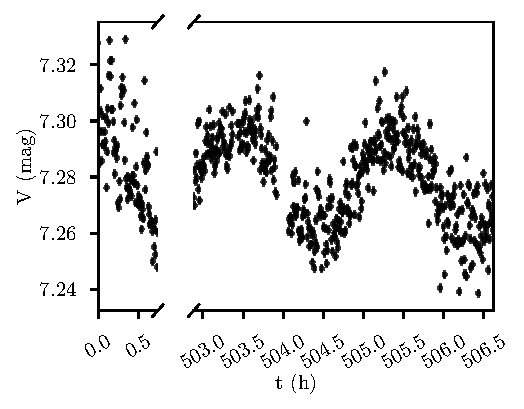
\includegraphics[width=\linewidth]{figs/rawmags.pdf}
	 	\caption{Photometry results for both observation nights}
	 	\label{fig:raw}
	 \end{figure}
	 \begin{figure}[t]
	 	\centering
	 	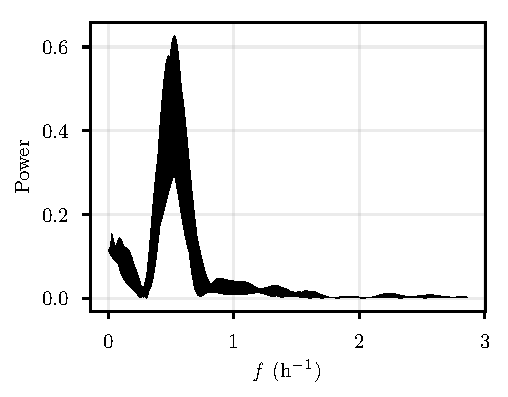
\includegraphics[width=\linewidth]{figs/power.pdf}
	 	\caption{Lomb-Scargle Periodogram. Peak is around \SI{0.53}{\per \hour}}
	 	\label{fig:power}
	 \end{figure}
 	\begin{figure}[t]
 		\centering
 		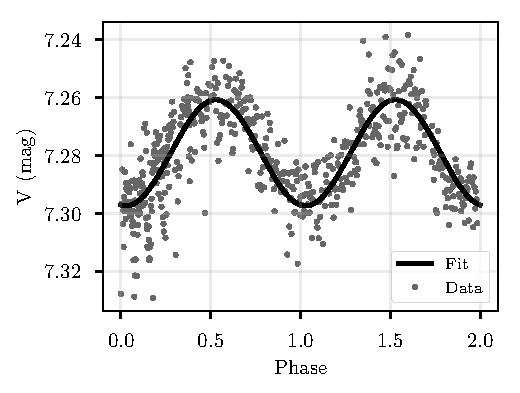
\includegraphics[width=\linewidth]{figs/fit.pdf}
 		\caption{Folded data with single-term Fourier series fit based on best frequency from Lomb-Scargle Periodogram. The magnitude errors are ignored due to their very small relative sizes to avoid visual clutter.}
 		\label{fig:fit}
 	\end{figure}
	
%________________________________________________________________________
	
%	Add here anything else you want to say, and summarize your results. This section should be very brief, not more than a couple of paragraphs
	\section{Conclusions}
	
	DQ Cephei is clearly variable over a period of \SI{1.89}{\hour}. We are happy with the precision our setup offered, but the variances in photometric magnitudes introduce a lot of systematic error into our system. The noise of our data is almost too large to notice the wave pattern. We trust the methods AIJ uses for differential photometry and the subsequent errors in that analysis, so we conclude that our telescope and CCD were the limiting agents in our analysis. 
	
	With that being said, our period analysis should still be reliable, because the variations in magnitudes all move around some mean (assuming Gaussian variations). For a variable star, we can suppose that the mean is varying, so as long as our variations are consistent, the periodogram methods will be accurate. This is why, despite different equipment, our period is exactly the same as the period from \citet{1971GCVS3.C......0K}. This periodogram is especially precise with the savvy algorithms developed for inconsistent time-series data since the analysis of \citet{1971GCVS3.C......0K}. This variance, though, causes issues with estimating the magnitude range of the star. While our model says DQ Cep ought to vary from \SIrange{7.26}{7.30}{mag} in V, we cannot say with confidence that this is more accurate than the magnitudes provided by \citet{1971GCVS3.C......0K}.
	
%________________________________________________________________________
	
	\section*{Acknowledgements}
	
	Thank you to Dr. Charles Kerton and Brandon Marshall for their guidance and assistance in this work.
	
	\medskip
	\bibliography{refs}
	
	
%________________________________________________________________________
	
	\onecolumngrid
	\appendix
	\section{Observation Log}

	\begin{table}[h!]
		\centering
		\caption{Observed 27 September 2017 by Miles Lucas}
\begin{tabular}{clclcccl}
	\hline
	Time  & File            & N Frames & Object & Filter &     Exposure     &      Camera Temp.      & Notes \\ \hline\hline
	0927/21:22 & DqCep\_V\_15s\_ &   100    & DQ Cep &   V    & \SI{15}{\second} & \SI{5}{\degreeCelsius} &  \\ \hline
\end{tabular}
		\label{table:log1}
	\end{table}

	\begin{table}[h!]
		\centering
		\caption{Observed 18 October 2017 by Miles Lucas and John Brandon}
\begin{tabular}{clclcccl}
	\hline
	Time  & File            & N Frames & Object & Filter &     Exposure     &      Camera Temp.      & Notes \\ \hline\hline
	1018/20:15 & DqCep\_V\_15s\_ &   482    & DQ Cep &   V    & \SI{15}{\second} & \SI{5}{\degreeCelsius} &  \\ \hline
\end{tabular}
		\label{table:log2}
	\end{table}
%________________________________________________________________________
	
	\section{Analysis Scripts}
	
	Please reference the jupyter notebook at \href{https://github.com/mileslucas/astro344l/blob/master/project/src/project.ipynb}{this github page}.
\end{document}
%
% ****** End of file aipsamp.tex ******
